\chapter{Experiments on fire alone}

\section{Recording and processing of stimuli}

A continuous 45-minute recording was acquired from a hearth fire using a Sony INS camera recording at 50 Hz. The scene was lit by a mixture of natural and artificial light and CCD gain was set to zero. Video was saved directly to the compressed AVCHD format at an initial resolution of 1024 by 768.

Before presentation, stimuli were cropped to 564 by 641 pixels, removing the background and most of the fireplace. Individual frames were decompressed and saved as bitmaps. 



\begin{figure}[htp]
\centering

\begin{subfigure}[b]{\textwidth}
\centering
                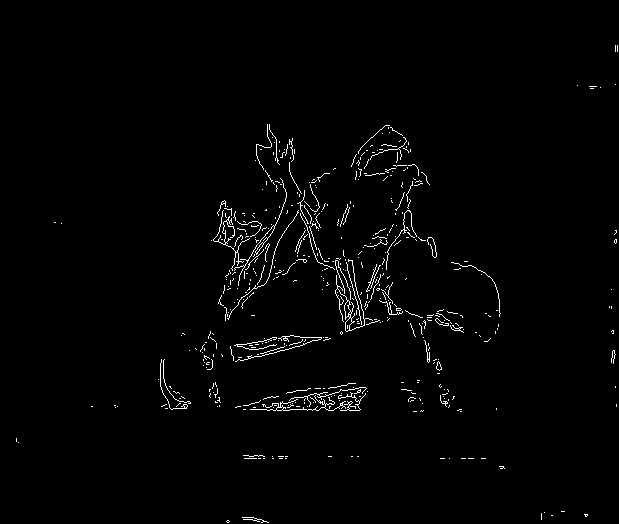
\includegraphics[width=12cm]{img/frame00000.png}
                \caption{Stimuli in original 1024 by 768 resolution.}
          
        \end{subfigure}

\begin{subfigure}[b]{\textwidth}
\centering
                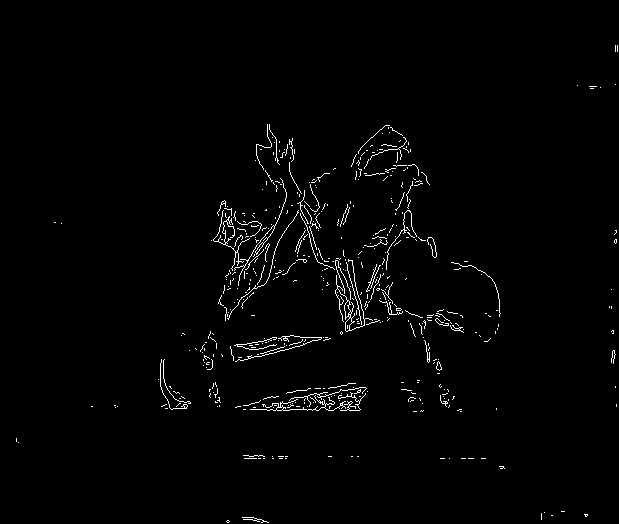
\includegraphics[width=12cm]{img/frame00000.png}
                \caption{Stimuli cropped to 564 by 641 pixels, as presented to subjects.}
          
        \end{subfigure}

\caption{Stimuli used in our visual search experiments.}
\end{figure}

\section{Experimental set-up}

Experiments were coded in MATLAB using Psychtoolbox. Video was displayed by loading bitmaps into video memory and manually displaying each one to the screen. This allowed precise control of frame rate.

Stimuli were displayed at 50 Hz on an INS monitor with a refresh rate of 100 Hz and a resolution of INS. The active video area subtended a visual angle of 14º; subjects used a chin-rest at a distance of 57 cm from the screen and were asked not to deviate their head angle from the vertical. Subjects were not requested to fixate, and the experiment took place in a darkened room.

All monitors used during these experiments were identically calibrated using a Cambridge Research Systems ColorCal or ColorCal MKII.


\section{Experiment 1: \textbf{search-ratio}}

\subsection{Methodology}

\paragraph{Stimuli}

A 1000-frame corpus of consecutive fire images was used.

\paragraph{Subjects}

12 subjects were recruited using a mailing list operated by University College London. All reported normal or corrected-to-normal vision.

\paragraph{Trial structure}

In each trial, a sample was presented first, followed by two tests. Subjects indicated which test they thought corresponded to the sample using the left arrow (first sample) and right arrow (second sample) keys. 

\paragraph{Factors}

Sample length (sL) was one of (10 25 50) frames, equivalently (0.2 0.5 1) seconds.
Ratio of sample to test was one of (1.2 1.4 1.6 1.8 2).

This gave the following sample lengths:
10-frame sample: 12 14  16 18 20 frames, 0.24, 0.28, 0.32, 0.36, 0.4 seconds
25-frame sample: 30 35 40 45 50 frames, 0.6,0.7,0.8, 0.9, 1 seconds
50-frame sample: 60    70    80    90   100 frames, 1.2,1.4,1.6,1.8,  2 seconds

There were 3*5 = 15 conditions.

\paragraph{Block structure}

25 training trials were presented first.

Sample length was varied across blocks. Target length was varied within blocks.

We presented 3 blocks, one corresponding to each target length, in random order. Subjects took a short break between blocks.

We used a total of 600 trials (40 trials per condition).

\subsection{Results}

\paragraph{Sample length}

We observed the following mean accuracies:

\begin{center}
\begin{tabular}{ r | l   }
\textbf{Sample length} & \textbf{Mean accuracy}\\
\hline
10 frames (0.2 s) & 0.728\\
 25 frames (0.5 s)&  0.704\\
 50 frames (1 s)&  0.687\\
\end{tabular}
\end{center}

Paired-sample $t$-tests revealed a significant accuracy drop between the 0.2 s samples and the 1 s samples ($p$<0.05) but not between any other pairs of levels. Subjects are more capable of matching longer samples.

\paragraph{Test/sample ratio}

The ratio by which the test was longer than the sample (which rises as the search space increases) had a significant effect on subject performance.

\begin{center}
\begin{tabular}{ r | l   }
\textbf{Test/sample ratio} & \textbf{Mean accuracy}\\
\hline
1.2 &  0.746\\
1.4 &  0.724\\
1.6 & 0.704\\
1.8 &  0.696\\
 2&  0.664\\
\end{tabular}
\end{center}

Paired-sample $t$-tests revealed significant differences between ratio=1.2 and each of the other levels; between ratio=1.8 and ratio=2 ($p<$0.05); and between ratio=1.4 and ratio=5 ($p<$0.01).

\paragraph{Learning rate}

We measured the subjects' learning rate by arranging the correct/incorrect responses in the order in which they were presented during the experimental run, blocking them into sequential groups of 20, and calculating the mean accuracy of each group. As shown in Fig. \ref{f:e1:learn}

\subsection{Discussion}

A two-factor repeated-measures ANOVA shows a highly significant effect of test/sample ratio ($p<$0.0001) but not of sample length ( ($p=$0.203) or of the ratio/sample length interaction ($p=$0.503). Neither is there an effect of absolute test length: see Fig. \ref{f:e1:tests}. The three sample length conditions ranged over three sets of test lengths which did not overlap at all; but, when re-expressed in terms of ratios, the effects on accuracy were consistent.

It is therefore the ratio between test and sample which determines the difficulty of the task\footnote{We use difficulty here as a proxy for accuracy, not to indicate the perceived ``hardness" of the task, which we did not measure.}, not the absolute lengths of either the target or the test.

 


\begin{figure}[htp]
\centering
\renewcommand{\arraystretch}{1.8}

      \begin{subfigure}[b]{\textwidth}
\begin{tabular}{ >{\bfseries}r | p{8cm}   }
& \textbf{Experiment 1}\\
\hline
  
	Design & 2AFC delayed match-to-sample (sample clip followed by two test clips)\\                   
  Stimuli & 1000-frame corpus \\
  Factors & sample length (10, 25, 50) frames or (0.2, 0.5, 1)seconds. \newline 
sample/test ratio (1.2 1.4 1.6 1.8 2).\\
  Block design & Sample length varied across blocks\newline
			Test length varied within blocks \newline
			15 conditions \newline
40 trials per condition \newline
600 trials \newline
25 training trials \\
\end{tabular}
\caption{Design summary.}
   \end{subfigure}

\begin{subfigure}[b]{\textwidth}
\centering
                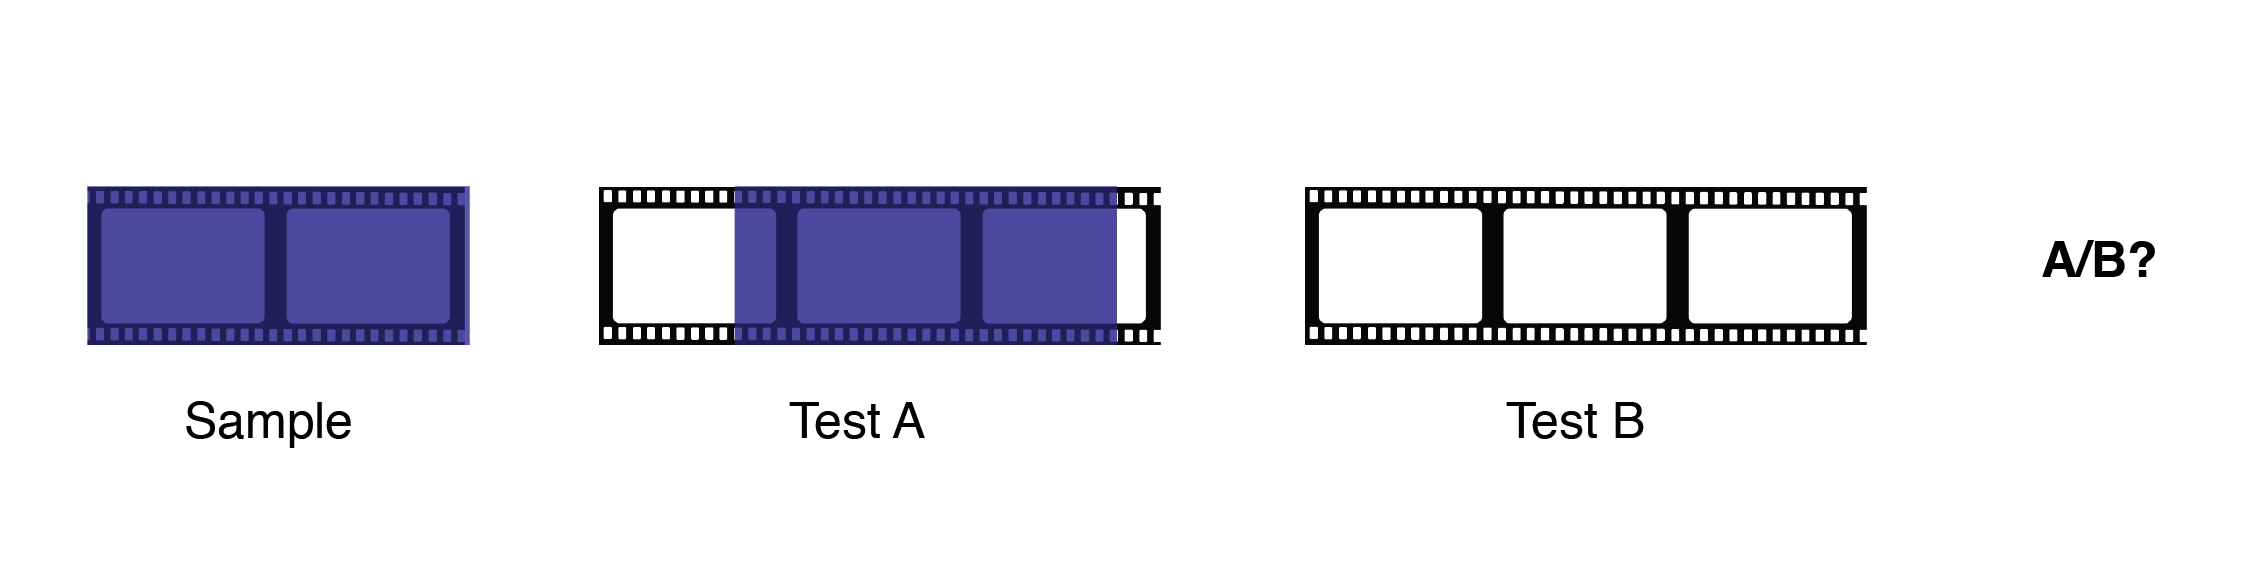
\includegraphics[width=12cm]{img/protocol_2afc.png}
                \caption{A short sample was followed by two longer tests, one of which contained the sample.}
         
        \end{subfigure}
\caption{Experiment 1: design summary and trial structure.}
\end{figure}


\begin{figure}[htp]
\centering
\begin{subfigure}[b]{\textwidth}
\centering
                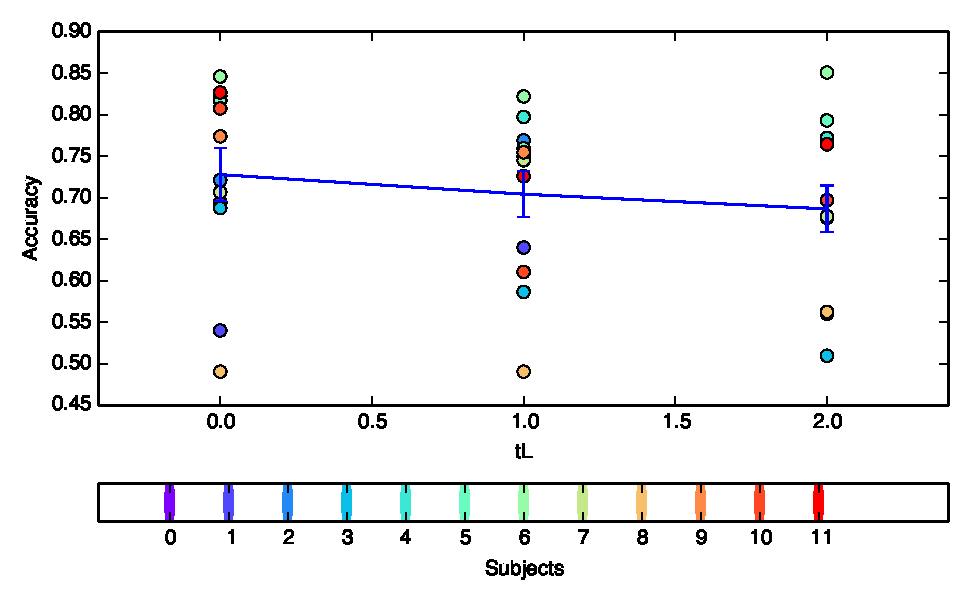
\includegraphics[width=12cm]{img/fig_fire3_correct_tL.pdf}
                \caption{Accuracy against sample length. Longer samples are more easily matched.}
          
        \end{subfigure}
\begin{subfigure}[b]{\textwidth}
\centering
                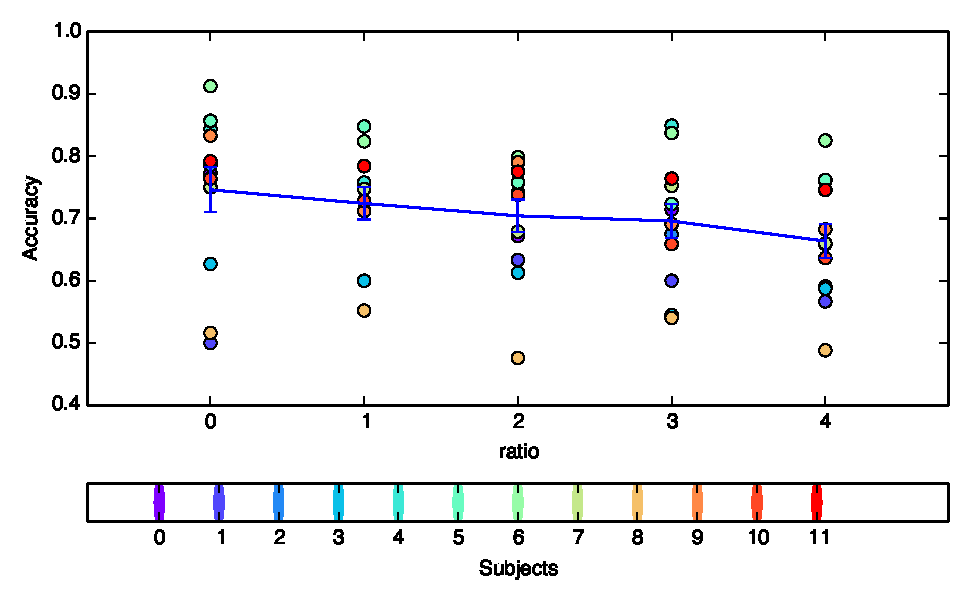
\includegraphics[width=12cm]{img/fig_fire3_correct_ratio.pdf}
                \caption{Accuracy against test/sample ratio. Longer tests render the sample harder to find.}
         
        \end{subfigure}
\caption{Experiment 1: the effects on accuracy of varying sample length, and test/sample ratio.}
\end{figure}

\begin{figure}[htp]
\centering
\begin{subfigure}[b]{\textwidth}
\centering
                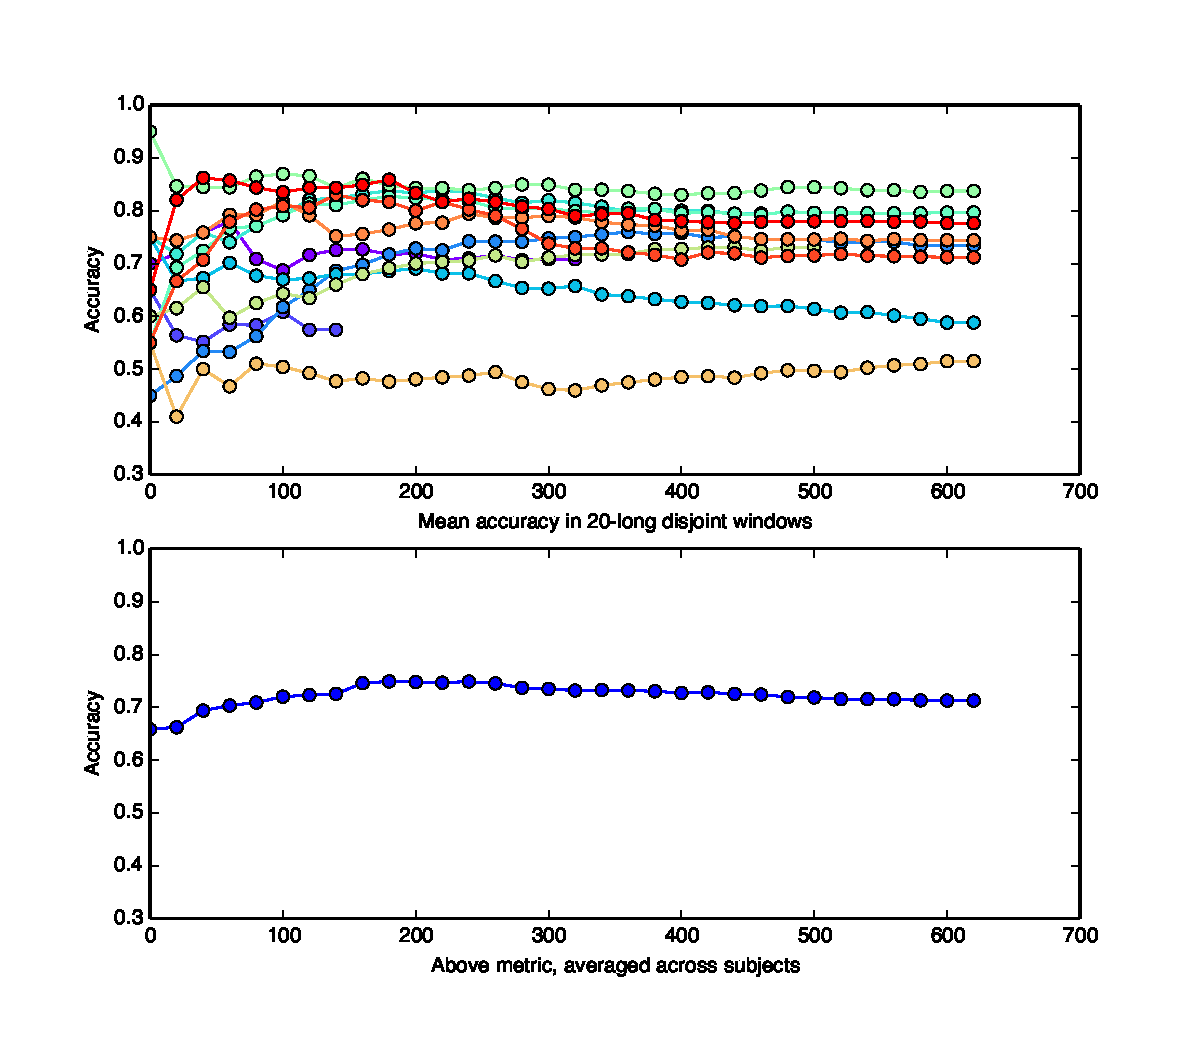
\includegraphics[width=12cm]{img/fig_fire3accuracyWalkingWindow.pdf}
                \caption{Learning: accuracy vs. trial number, blocked into groups of 20.}
      		\label{f:e1:learn}
        \end{subfigure}
\caption{Experiment 1: the effects on accuracy of varying sample length, and test/sample ratio. As throughout this document, error bars are 1 SEM.}
\end{figure}